\documentclass[11pt]{article}
\usepackage[scaled=0.92]{helvet}
\usepackage{geometry}
\geometry{letterpaper,tmargin=1in,bmargin=1in,lmargin=1in,rmargin=1in}
\usepackage[parfill]{parskip} % Activate to begin paragraphs with an empty line rather than an indent %\usepackage{graphicx}
\usepackage{amsmath,amssymb, mathrsfs, dsfont}
\usepackage{tabularx}
\usepackage[font=footnotesize,labelfont=bf]{caption}
\usepackage{graphicx}
\usepackage{xcolor}
%\usepackage{ulem}
%\usepackage[linkbordercolor ={1 1 1} ]{hyperref}
%\usepackage[sf]{titlesec}
\usepackage{natbib}
\usepackage{../../Tianpei_Report}

%\usepackage{appendix}
%\usepackage{algorithm}
%\usepackage{algorithmic}

%\renewcommand{\algorithmicrequire}{\textbf{Input:}}
%\renewcommand{\algorithmicensure}{\textbf{Output:}}



\begin{document}
\title{Lecture 3: Finite Markov Decision Process (MDP)}
\author{Tianpei Xie}
\date{ Aug 1st., 2022 }
\maketitle
\tableofcontents
\newpage
\section{Markov Decision Process}
\begin{figure}
\begin{minipage}[t]{1\linewidth}
  \centering
  \centerline{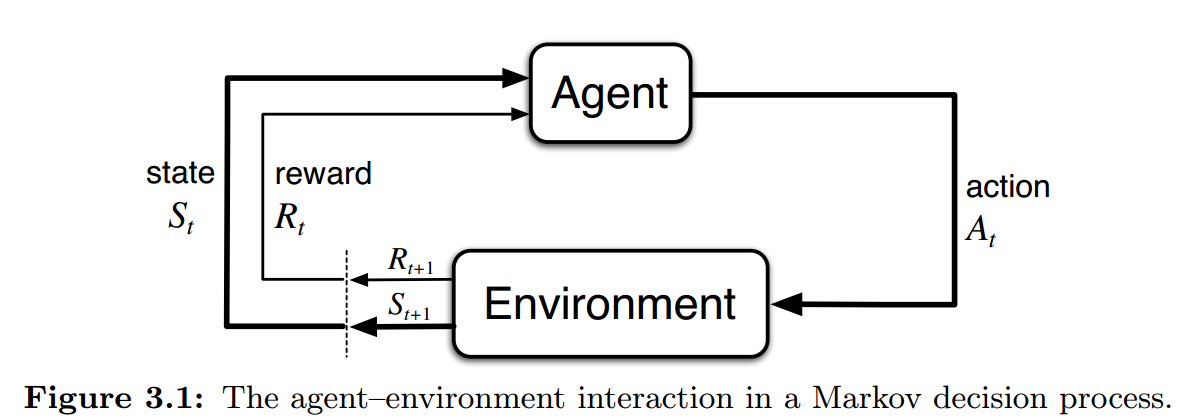
\includegraphics[scale = 0.3]{mdp.png}}
\end{minipage}
\caption{\footnotesize{\textbf{Markov Decision process formulation}.  \citep{sutton2018reinforcement}}}
\label{fig: mdp}
\end{figure}

\textbf{\emph{Markov Decision Processes}} (MDPs) are a classical formalization of sequential decision making, where actions influence not just immediate rewards, but also subsequent situations, or states, and through those future rewards. Thus MDPs involve delayed reward and the need to tradeoff immediate and delayed reward.  MDPs are meant to be a straightforward framing of the problem of learning from interaction to achieve a goal. There are several aspects in the formulation:
\begin{itemize}
\item \textbf{agents}: The learner and decision maker;
\item \textbf{environment}: The thing agent interacts with, comprising everything outside the agent;
\item the agent and environment interact at each of a sequence of \textbf{discrete time steps} $t=1,2,\ldots,$;
\item At each time step $t$, the agent receives some representation of the environment’s \textbf{state}, $S_t \in  \cS$; state is the \emph{basis} on which the action is taken
\item and on that basis selects an \textbf{action}, $A_t \in \cA(s)$. Action signals represent \emph{choices} made by the agent.
\item One time step later $t+1$, in part as a consequence of its action, the agent receives a numerical \textbf{reward}, $R_{t+1} \in \cR \subset \bR$, and finds itself in a \textbf{new state}, $S_{t+1}$; The reward defines the \emph{\textbf{objective}} of learning and the \emph{\textbf{goal}} of agent. 
\item For finite MDP, i.e. $(\cS, \cA, \cR)$ are finite sets,  the \textbf{dynamic function} is defined as $p: \cS \times \cA \times \cS \times \cR \rightarrow [0,1]$, $p(s', r| s, a):= P( S_{t+1}=s',R_{t+1}=r| S_{t}=s, A_{t}=a)$ for all $s,s' \in \cS, a\in \cA(s), r\in \cR$. The function $p$ defines the \emph{\textbf{dynamics}} of the MDP. ($|$ in p is borrowed from conditional prob but the function determined by all of inputs)
\end{itemize} This formulation is called \emph{Markov Decision Process} since the future states and rewards are only dependent on the immediately preceding state and action, not past histories.  Figure \ref{fig: mdp} illustrate the relations between these aspects. We can fully represent a MDP as a tuple $(\cS, \cA, \cR, p(\cdot|\cdot))$.

The formulation of MDP has high requirement on definition of {\emph{state}}. The state must include information about \emph{all aspects of the past agent-environment interaction} that make a difference for the future. The \emph{state transition probablity} can be obtained via marginalization
\begin{align*}
p(s' | s, a) &= \sum_{r\in \cR}p(s', r | s, a).
\end{align*} The \emph{expected rewards} for state-action pair $r: \cS \times \cA \rightarrow \cR$ can be obtained 
\begin{align}
r(s,a) &= \E{p}{R_{t+1}|S_{t}=s, A_{t}=a} = \sum_{r\in \cR}r \;\sum_{s'\in \cS}p(s', r| s, a). \label{eqn: expected_rewards_state_action}
\end{align}The \emph{expected rewards} for state-action-next-state pair $r: \cS \times \cA \times \cS \rightarrow \cR$ can be obtained 
\begin{align*}
r(s,a, s') &= \E{p}{R_{t+1}|S_{t+1}=s', S_{t}=s, A_{t}=a} = \sum_{r\in \cR}r \;\frac{p(s', r| s, a)}{p(s' | s, a)}
\end{align*}

The MDP framework is abstract and flexible and can be applied to many different problems in many different ways. In general, actions can be any decisions we want to learn how to make, and the states can be anything we can know that might be useful in making them. In particular, the boundary between agent and environment is typically not the same as the physical boundary of a robot’s or animal’s body. Usually, the boundary is drawn closer to the agent than that. Rewards, too, presumably are computed inside the physical bodies of natural and artificial learning systems, but are considered external to the agent.

The general rule we follow is that \emph{anything that \textbf{cannot be changed arbitrarily} by the agent is considered to be \textbf{outside} of it} and thus part of its environment. We do not assume that everything in the environment is unknown to the agent. For example, the agent often knows quite a bit about how its rewards are computed as a function of its actions and the states in which they are taken. But we always consider the\emph{ reward computation to be \textbf{external}} to the agent because it defines the task facing the agent and thus must be beyond its ability to change arbitrarily. In fact, in some cases the agent may know everything about how its environment works and still face a diffcult reinforcement learning task, just as we may know exactly how a puzzle like Rubik’s cube works, but still be unable to solve it. \textbf{The agent-environment boundary represents the limit of the agent’s absolute control, not of its knowledge}. In practice, the agent–environment boundary is determined once one has selected particular states, actions, and rewards, and thus has identified a specific decision making task of interest.

\section{Goals and Rewards}
In reinforcement learning, the \textbf{purpose or goal} of the agent is formalized in terms of a special signal, called the \emph{\textbf{reward}}, passing from the environment to the agent. Informally, the agent’s goal is to maximize the total amount of reward it receives. We can clearly state this informal idea as the \emph{\textbf{reward hypothesis}}:

 "That all of what we mean by goals and purposes can be well thought of as
the \textbf{maximization} of the \emph{\textbf{expected}} value of the \emph{\textbf{cumulative sum}} of a received \textbf{scalar} signal (called reward)."

The use of a \emph{reward signal} to formalize the \emph{idea of a goal} is one of the most \textbf{distinctive features of reinforcement learning}. Note that the reward signal is \underline{\textbf{not}} the place to impart to the agent prior knowledge about \underline{how to achieve what we want it to do}. If the winning is the goal, then achieving subgoals are not considered as rewards, since the agents may stop when achieving the subgoal. 

In many real-world examples, however, the reward hypothesis may not hold. For instance, if the goal is to achieve the best outcome under worst case situations, then simply maximing the rewards may not yield the good solution. Similar case such as risk-sensitive/avert examples also requires us to find solution that may not be the best in terms of cumulative rewards but avoids the worst situations.  Also, sometimes, if the goal is very far away, and solving sub-problems may still make sense to achive the end results, 

\section{Returns and Episodes}
The \textbf{return} is defined as the \emph{cumulative rewards in the long run/ in future}. In general, we seek to maximize the \textbf{\emph{expected return}}, where the \textbf{return}, denoted $G_t$, is
defined as some specific function of the reward sequence. 
\begin{align*}
G_{t} &= \sum_{\tau > t}R_{\tau}.
\end{align*}
In applications, where a final state at $T$ can be observed and after that, the enviroment and agents will be reset to inital state,  the agent-environment interaction breaks naturally into \emph{subsequences}, which we call \textbf{episodes}. Examples include games such as chess, maze et al. Each episode ends in a special
state called \textbf{the terminal state}, followed by a reset to a standard starting state or to a sample from a standard distribution of starting states. Tasks
with episodes of this kind are called \textbf{episodic tasks}. In episodic tasks we sometimes need to distinguish the set of all nonterminal states, denoted $\cS$, from the set of all states plus the terminal state, denoted $\cS+$. The time of termination, $T$, is a random variable that normally varies from episode to episode. For episodic tasks,  the return is finite $G_{t} = \sum_{t}^{T}R_{\tau}$.

On the other hand, in many cases the agent–environment interaction does not break naturally into identifiable episodes, but goes on continually \emph{without limit}. For example, this would be the natural way to formulate an on-going process-control task, or an application to a robot with a long life span. We call these \textbf{continuing tasks}. The return for continuing task can be infinite. So, in order to compute finite expectation of returns, we usually apply \textbf{discounts} $\gamma$ for future rewards based on the time passing. The \textbf{\emph{discounted return}} is formulated as below
\begin{align}
G_{t} &= \sum_{\tau > t}\gamma^{\tau}R_{\tau} < \infty \nonumber\\
&= R_{t+1} + \gamma\,G_{t+1}, \label{eqn: discount_return}
\end{align} where $\gamma \in [0,1]$. The \textbf{discount rate} $\gamma$ determines the \emph{present} value of \emph{future rewards}. Then $\gamma =0$, $G_{t} = R_{t+1}$, i.e. the short-sighted returns. If $\gamma \rightarrow 1$, we have the far-sighted returns, where the return objective takes future rewards into account more strongly. 

We can combine the notion of returns for episodic and continuing task as follows:
\begin{align}
G_{t}&= \sum_{\tau = t+1}^{T}\gamma^{\tau-t-1}R_{\tau}.  \label{eqn: return} \\
&=R_{t+1} + \gamma\,G_{t+1}  \nonumber
\end{align} Note that we can allow $T=\infty$ or $\gamma=1$ but not both. To convert an episodic task into continuing task, we can define an absorbing state that transitions only to to itself and generates zero rewards. 


\section{Policies and Value Functions}
The policy and value functions are defined as follows:
\begin{itemize}
\item Formally, a \emph{\textbf{policy}} is a mapping from \emph{states} to probabilities of selecting each possible \emph{action}. Define $\pi: \cS \rightarrow \cP(\cA)$ as the policy function. $\pi(a|s) = P(A_t=a | S_t=s)$  is the probability that $A_t = a$ if $S_t = s$.  Like $p$, $\pi$ is an ordinary function; the “$|$” in the middle of $\pi(a|s)$ merely reminds that it defines a probability distribution over $a \in \cA(s)$ for each $s \in \cS$. Reinforcement learning methods specify how the agent’s policy is \emph{changed} as a result of its experience. 
\begin{itemize}
\item \textbf{deterministic policy}: when $\pi: \cS \rightarrow \cA$ is a deterministic function, i.e. given a state, the policy $\pi(a|s) = \ind{a}$ only assign a fixed action $a$ from the state $s$.

\item \textbf{stochastic policy}: when $\pi(a|s) = P(A_t=a | S_t=s)$, i.e. the policy randomly select an action according to a probability distribution $\pi(a|s)$
\end{itemize}

\item The \emph{\textbf{value function (state-value function) }}$v_{\pi}: \cS \rightarrow \bR$ of \textbf{a \emph{state} $s$ under a \emph{policy} $\pi$}, denoted $v_{\pi}(s)$, is the \emph{\textbf{expected future return}} when \emph{starting} in $s$ and \emph{following} $\pi$ thereafter. 
\begin{align}
v_{\pi}(s) &:= \E{\pi}{G_{t} | S_{t} = s}  \label{eqn: value_fun}\\
&= \E{\pi}{\sum_{\tau=0}^{\infty}\gamma^{\tau}R_{\tau+t+1} \Big| S_{t} = s}, \quad \gamma \in [0,1), \forall\, s\in \cS, \nonumber
\end{align} where $\E{\pi}{\cdot}$ denotes the expected value of a random variable given that the agent follows policy $\pi$, and $t$ is any time step.

\item The \emph{\textbf{action-value function for policy $\pi$}}. denoted $q_{\pi}(s,a)$, is the \emph{\textbf{expected return}} starting from $s$, taking the action $a$, and thereafter following policy $\pi$:
\begin{align}
q_{\pi}(s, a) &:= \E{\pi}{G_{t} | S_{t} = s, \;A_{t}=a}  \label{eqn: value_action_state_fun}\\
&=\E{\pi}{\sum_{\tau=0}^{\infty}\gamma^{\tau}R_{\tau+t+1} \Big| S_{t} = s, \, A_{t} = a} , \nonumber
\end{align}
\end{itemize}
Note that the \emph{policy} $\pi$ is the  function of \textbf{current state value only}. It does not depends on previous actions, states or time.  The value function reflects an estimate of \emph{how good} it is for the agent to be in a given state (or how good it is to perform a given action in a given state). The notion of “how good” here is defined in terms of future rewards that can be expected, or, to be precise, in terms of \emph{expected return}.  Both $v_{\pi}(s)$ and $q_{\pi}(s,a)$ can be estimated via averaging from samples with Monte Carlo methods. 

See following exercises.  
\begin{exercise} Give an equation for $v_{\pi}$ in terms of $q_{\pi}$ and $\pi$.
\end{exercise}
\begin{solution} Note that $v_{\pi}$ can be obtained directly via marginalization of $q_{\pi}$
\begin{align}
v_{\pi}(s) &:= \E{\pi}{G_{t} | S_{t} = s} \nonumber\\
&= \E{\pi}{\E{\pi}{G_{t} | S_{t} = s, \;A_{t}=a}} \nonumber\\
&=\E{\pi}{q_{\pi}(s, A_{t}) | S_{t}=s}\label{eqn: value_fun_by_value_action2}\\
&= \sum_{a}\pi(a|s)q_{\pi}(s, a).\;\;\QEDA   \label{eqn: value_fun_by_value_action}
\end{align} 
\end{solution}

\begin{exercise} Give an equation for $q_{\pi}$ in terms of $v_{\pi}$ and the four-argument $p$
\end{exercise}
\begin{solution}
\begin{align}
q_{\pi}(s, a) &:= \E{\pi}{G_{t} | S_{t} = s, \;A_{t}=a}\nonumber\\
&(\text{since } G_{t} = R_{t+1} + \gamma\,G_{t+1}) \nonumber\\
&= \E{\pi}{R_{t+1} | S_{t} = s, \;A_{t}=a} + \gamma\,\E{\pi}{G_{t+1} | S_{t} = s, \;A_{t}=a} \nonumber\\
&= \sum_{s'}\sum_{r}p(s', r| s, a)r + \gamma\sum_{s'}\sum_{r}p(s', r| s, a) \E{\pi}{G_{t+1}| S_{t+1}=s', S_{t} = s, \;A_{t}=a}\nonumber\\
&= \sum_{s'}\sum_{r}p(s', r| s, a)\brac{r + \gamma\,\E{\pi}{G_{t+1}| S_{t+1}=s', S_{t} = s, \;A_{t}=a}}\nonumber\\
&\text{by Markov property}\nonumber\\
&= \sum_{s'}\sum_{r}p(s', r| s, a)\brac{r + \gamma\,\E{\pi}{G_{t+1} | S_{t+1}=s'}}\nonumber\\
&(\text{since }v_{\pi}(s') := \E{\pi}{G_{t+1} | S_{t+1} = s'} \nonumber\\
&= \underline{\sum_{s'}\sum_{r}p(s', r| s, a)\brac{r + \gamma\,v_{\pi}(s')}} \label{eqn: value_action_fun_by_value}\\
&=  \underline{\E{}{R_{t+1} + \gamma\,v_{\pi}(S_{t+1})| S_{t}=s, A_{t} = a}}.\;\; \QEDA \label{eqn: value_action_fun_by_value2}
\end{align}  
\end{solution}
\subsection{Bellman equation}
A fundamental property of value functions used throughout reinforcement learning and dynamic programming is that they satisfy \textbf{\emph{recursive} relationships} similar to that which we have already established for the return. 

From above equation \eqref{eqn: value_action_fun_by_value} and substitue equation \eqref{eqn: value_fun_by_value_action} we can find action-value function
\begin{align}
q_{\pi}(s, a) &= \sum_{s'}\sum_{r}p(s', r| s, a)\brac{r + \gamma\,v_{\pi}(s')} \nonumber\\
&= \underline{\sum_{s', r}p(s', r|s,a)\brac{r+ \gamma \sum_{a'}\pi(a'|s')q_{\pi}(s', a')}}, \quad \forall\,\; s\in \cS, \; a\in \cA(s) \label{eqn: bellman_eqn_value_action}\\
&= \underline{\E{}{R_{t+1} + \gamma q_{\pi}(S_{t+1}, A_{t+1}) | S_{t}=s, A_{t}=a}} \label{eqn: bellman_eqn_value_action2}
\end{align} Similarly, the derivation of equation \eqref{eqn: value_fun_by_value_action} can be seen as 
\begin{align}
v_{\pi}(s) &:= \E{\pi}{G_{t} | S_{t} = s} \nonumber\\
&(\text{since } G_{t} = R_{t+1} + \gamma\,G_{t+1})  \nonumber\\
&= \E{\pi}{R_{t+1}  + \gamma\,G_{t+1} | S_{t} = s}  \nonumber\\
&= \E{A_{t}, R_{t+1}, S_{t+1}}{\E{\pi}{R_{t+1}  + \gamma\,G_{t+1} | S_{t} = s, A_{t}=a, R_{t+1}=r, S_{t+1}=s'}}  \nonumber\\
&= \E{A_{t}, R_{t+1}, S_{t+1}}{r  + \gamma\,\E{\pi}{G_{t+1} | S_{t} = s, A_{t}=a, R_{t+1}=r, S_{t+1}=s'}}  \nonumber\\
&\text{by Markov property} \nonumber\\
&= \sum_{a}\pi(a|s)\sum_{s'}\sum_{r}p(s', r| s, a)\brac{r + \gamma \E{\pi}{G_{t+1} | S_{t+1} = s'}} \nonumber\\
&=  \underline{\sum_{a}\pi(a|s)\sum_{s'}\sum_{r}p(s', r| s, a)\brac{r + \gamma v_{\pi}(s')}}, \quad \forall\,\; s\in \cS \label{eqn: bellman_eqn_value}\\
&= \underline{\E{}{R_{t+1}  + \gamma\,v_{\pi}(S_{t+1}) | S_{t} = s}} \label{eqn: bellman_eqn_value2}
\end{align}

Both \eqref{eqn: bellman_eqn_value_action} and \eqref{eqn: bellman_eqn_value} are referred as the \emph{\textbf{Bellman equation}} for  action-value function $q_{\pi}(s, a)$ and value function  $v_{\pi}(s)$, respectively. Bellman equation states that for any policy $\pi$ and any state $s$, the following consistency condition holds between the \emph{value} of $s$ and the \emph{value} of its possible \emph{successor states}; similarly for the action-value function:
\begin{align}
v_{\pi}(s) &= r(s) + \gamma \sum_{s'}\brac{\sum_{a}\pi(a|s)p(s'| s, a)}v_{\pi}(s'), \quad \forall\,\; s\in \cS \label{eqn: bellman_eqn_value3}\\
q_{\pi}(s, a) &=  r(s,a) + \gamma\sum_{s'}\sum_{a'}\brac{\pi(a'|s')p(s'|s,a)}q_{\pi}(s', a'), \quad \forall\,\; s\in \cS, \; a\in \cA(s) \label{eqn: bellman_eqn_value_action2}
\end{align} where $r(s,a) := \E{\pi}{R_{t+1} | S_{t} = s, \;A_{t}=a}$ from \eqref{eqn: expected_rewards_state_action} and $r(s) =  \E{\pi}{r(s,a)| s} = \sum_{a}\pi(a|s)r(s,a)$. The Bellman equation states that the \textbf{value} of the \emph{start state} must equal the (discounted) \textbf{value} of the \textbf{expected next state} (the second term), \emph{plus} the \textbf{expected reward} \emph{along the way} (first term). 

\begin{theorem}
For any finite state MDP, the Bellman equation in \eqref{eqn: bellman_eqn_value} has an unique solution.
\end{theorem}  Since \eqref{eqn: bellman_eqn_value2} is a system of $|\cS|$ \textbf{linear equations} with $|\cS|$ unknown values, there exists an unique solution. 

\begin{figure}
\begin{minipage}[t]{1\linewidth}
  \centering
  \centerline{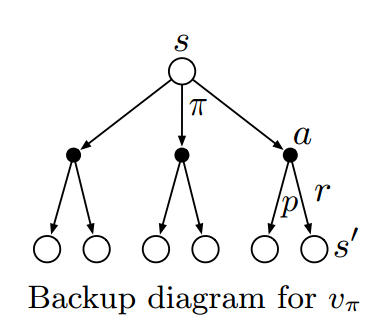
\includegraphics[scale = 0.3]{backup_diagram.png}}
\end{minipage}
\caption{\footnotesize{\textbf{backup diagram}.  \citep{sutton2018reinforcement}}}
\label{fig: backup_diagram}
\end{figure}

The Bellman equation can be visualized via a diagram in Figure \ref{fig: backup_diagram}. We call this diagrams \emph{\textbf{backup}} \emph{\textbf{diagrams}} because they diagram relationships that form the basis of the \emph{update} or \emph{backup} operations that are at the heart of reinforcement learning methods. These operations transfer value information \emph{back to a state} (or a state–action pair) from \emph{its successor states} (or state–action pairs). 

From Bellman equation we can see that the aggregate statistics on Markov network can be computed recursively via random walk. 

\subsection{Optimal Policy and Optimal Value Function}
Value functions define a partial ordering over policies. A policy $\pi$ is defined to be \emph{better} than or \emph{equal to} a policy $\pi^{'}$ if its expected return is greater than or equal to that of $\pi^{'}$ for all states. In other words, $\pi \ge \pi^{'}$ if and only if $v_{\pi}(s) \ge v_{\pi^{'}}(s)$ for all $s \in \cS$. \textbf{There is always at least one policy that is better than or equal to all other policies}. This is an \emph{\textbf{optimal policy}}. 

Note that if $v_{\pi_{1}}(s_{1}) \ge v_{\pi_{2}}(s_{1})$ and $v_{\pi_{1}}(s_{2}) \le v_{\pi_{2}}(s_2)$, then we can define a new policy $\pi_{3} = \pi_{1}$ if $s=s_{1}$ and $\pi_{3} = \pi_{2}$ if $s=s_{2}$ so that $\pi_{3} \ge \pi_{1}$ and $\pi_{3} \ge \pi_{2}$. For finite state MDPs, there always exists an optimal policy. Also even for finite state MDPs, \textbf{the optimal policy is not guaranteed to be unique}. 

Denote the optimal policy as $\pi_{*}$. They share the \emph{same state-value function}, called the \textbf{optimal state-value function}, denoted $v_{*}$, and defined as
\begin{align}
v_{*}(s) &:= v_{\pi_{*}}(s) \nonumber\\
&= \max_{\pi}v_{\pi}(s), \quad s\in \cS  \label{eqn: optimal_val}
\end{align} 
Optimal policies also share the same \textbf{optimal action-value function}, denoted $q_{*}$, and defined as 
\begin{align}
q_{*}(s, a) &:= q_{\pi_{*}}(s, a) \nonumber\\
&= \max_{\pi}q_{\pi}(s, a), \quad s\in \cS, \;\; a\in \cA(s)  \label{eqn: optimal_action_val}\\
&= \E{}{R_{t+1} + \gamma v_{*}(S_{t+1}) | S_{t} = s, \, A_{t} = a}  \label{eqn: optimal_action_val2}
\end{align} 

Because $v_{*}$ is the value function for a policy, it must satisfy the self-consistency condition given by the Bellman equation for state values \eqref{eqn: bellman_eqn_value}. Since $v_{*}$ is the optimal value function, the Bellman equation can be reformulated as below
\begin{align}
v_{*}(s)&= \max_{a\in \cA(s)}q_{\pi_{*}}(s, a) \nonumber\\
&= \max_{a\in \cA(s)}\E{\pi_{*}}{G_{t} | S_{t}=s, \, A_{t}=a} \nonumber\\
&= \max_{a\in \cA(s)}\E{\pi_{*}}{R_{t+1} + \gamma G_{t+1} | S_{t}=s, \, A_{t}=a} \nonumber\\
&= \underline{\max_{a\in \cA(s)}\E{}{R_{t+1} + \gamma v_{*}(S_{t+1}) | S_{t}=s, \, A_{t}=a}} \label{eqn: bellman_eqn_optimal_value1}\\
&= \underline{\max_{a\in \cA(s)}\sum_{s'}\sum_{r}p(s', r|s, a)\brac{r + \gamma v_{*}(s')}} \quad s\in \cS \label{eqn: bellman_eqn_optimal_value2}\\
&= \max_{a\in \cA(s)}\brac{r(s, a) + \gamma \sum_{s'}p(s'|s, a)v_{*}(s')} \label{eqn: bellman_eqn_optimal_value3}
\end{align}  \eqref{eqn: bellman_eqn_optimal_value1}, \eqref{eqn: bellman_eqn_optimal_value3} and  \eqref{eqn: bellman_eqn_optimal_value2} are three forms of \textbf{Bellman optimality equations} for $v_{*}$. Note that in the equation above, the \textbf{optimal value function does not depend on the the policy} $\pi$. In other words, multiple optimal policies share the same optimal value function. For finite MDPs, although the optimal policy $\pi_{*}$ is not unique, the \emph{optimal value function} $v_{*}$ is \emph{\textbf{unique}} and is determined by the Bellman equation  \eqref{eqn: bellman_eqn_optimal_value3} or \eqref{eqn: bellman_eqn_optimal_value2}.

\begin{theorem}
For finite MDP, the Bellman optimality equation \eqref{eqn: bellman_eqn_optimal_value2} for $v_{*}$ has a unique solution. 
\end{theorem} Same as the before, the Bellman optimality equation in \eqref{eqn: bellman_eqn_optimal_value2} is a system of $|\cS|$ equations with $|\cS|$ unknowns. 

The \emph{Bellman optimality equation} for the \emph{optimal action-value function} is 
\begin{align}
q_{*}(s, a) &=  \E{}{R_{t+1} + \gamma v_{*}(S_{t+1}) | S_{t} = s, \, A_{t} = a} \nonumber\\
&=\underline{\E{}{R_{t+1} + \gamma  \max_{a'\in \cA(s)}q_{*}(S_{t+1}, a')  \Big| S_{t} = s, \, A_{t} = a}}  \label{eqn: bellman_eqn_optimal_value_action3}\\
&= \underline{\sum_{s'}\sum_{r}p(s', r|s, a)\brac{r + \gamma  \max_{a'\in \cA(s)}q_{*}(s', a')}} \label{eqn: bellman_eqn_optimal_value_action} \\
&= r(s, a) +  \gamma \sum_{s'}p(s'| s, a)\max_{a' \in \cA(s)}q_{*}(s', a') \label{eqn: bellman_eqn_optimal_value_action2}
\end{align}



The backup diagrams in the Figure \ref{fig: backup_diagram_bellman_opt} show graphically the spans of future states and actions considered in the Bellman optimality equations for $v_{*}$ and $q_{*}$. These are the same as the backup diagrams for $v_{\pi}$ and $q_{\pi}$ presented earlier except that arcs have been added at the agent’s choice points to represent that the maximum over that choice is taken rather than the expected value given some policy. The backup diagram on the left graphically represents the Bellman optimality equation \eqref{eqn: bellman_eqn_optimal_value2} and the backup diagram on the right graphically represents \eqref{eqn: bellman_eqn_optimal_value_action}.

\begin{figure}
\begin{minipage}[t]{1\linewidth}
  \centering
  \centerline{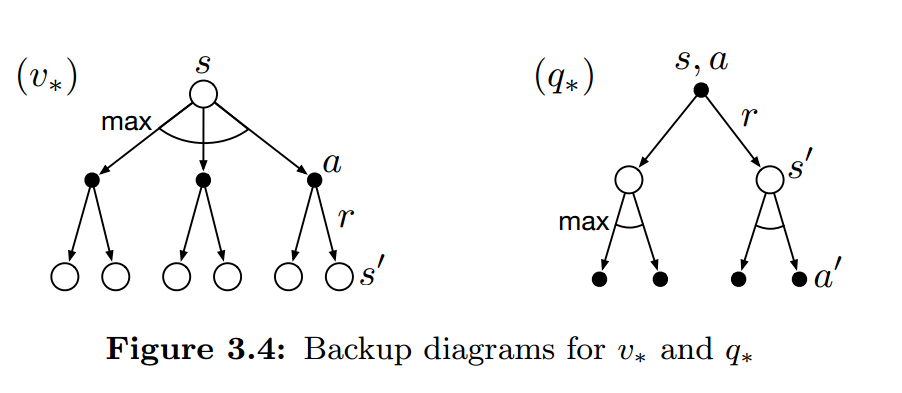
\includegraphics[scale = 0.3]{Bellman_eqn_opt.png}}
\end{minipage}
\caption{\footnotesize{\textbf{backup diagram for $v_{*}$ and $q_{*}$}.  \citep{sutton2018reinforcement}}}
\label{fig: backup_diagram_bellman_opt}
\end{figure}

Given the optimal value $v_{*}$ for each state, an \textbf{optimal policy} can be obtained by constructing a \emph{greedy} policy: $\pi(a|s) = 0$ for all $a \not\in \cA_{*}(s)$, where $$\cA_{*}(s):=\argmax_{a\in \cA(s)}\sum_{s'}\sum_{r}p(s', r|s, a)[r + \gamma v_{*}(s')]$$ is a set of actions that reach the maximum in the Bellman equation \eqref{eqn: bellman_eqn_optimal_value2}. This is a \emph{greedy policy} since it selects actions based only on their short-term consequences. This is an \textbf{one-step search}. If you have the optimal value function, $v_{*}$, then the actions that appear best after a one-step search will be optimal actions.  Although the (optimal) value function $v_{*}$ is used to evaluate the short-term consequences, a greedy policy is actually optimal in the long-term sense. The \emph{optimal value function} encodes the \emph{reward} consequences of \underline{all possible future behavior}. $v_{*}$ stores the optimal expected long-term return locally and is immediately available for each state. 

Based on the greedy deterministic optimal policy $\pi_{*}$ constructed as above, we can also derive the Bellman optimality equation based on Bellman equation in \eqref{eqn: bellman_eqn_value}:
\begin{align*}
v_{*}(s) = v_{\pi_{*}}(s) &= \sum_{a}\pi_{*}(a|s)\sum_{s'}\sum_{r}p(s', r| s, a)\brac{r + \gamma v_{\pi_{*}}(s')}, \quad \forall\,\; s\in \cS \\
&(\text{consider a deterministic optimal policy } \pi_{*} = \ind{A_{t} = a \in \cA_{*}(s)})\\
&= \max_{a \in \cA}\sum_{s'}\sum_{r}p(s', r| s, a)\brac{r + \gamma v_{*}(s')}
\end{align*}



Given the optimal action-value $q_{*}$  choosing optimal actions is even easier. With $q_{*}$, the agent does not even have to do a one-step-ahead search: for any state $s$, it can simply find any action that maximizes $q_{*}(s,a)$. The action-value function effectively \emph{caches} the \emph{results of all one-step-ahead searches}. It provides the optimal expected long-term return as a value that is locally and immediately available for each state–action pair.

Explicitly solving the Bellman optimality equation provides one route to finding an optimal policy, and thus to solving the reinforcement learning problem. In practice, this brute-force search rarely works since the number of states $|\cS|$ is usually extremely large for real-world problems, thus making the solution finding very inefficient. Moreover, this solution relies on at least three assumptions that are rarely true in practice: 
\begin{enumerate}
\item we accurately know the \emph{dynamics} of the environment;
\item we have enough\emph{ computational resources} to complete the computation of the solution;
\item the Markov property.
\end{enumerate} For the kinds of tasks in which we are interested, one is generally not able to implement this solution exactly because various combinations of these assumptions are violated. 

Many different decision-making methods can be viewed as ways of \textbf{approximately} solving the Bellman optimality equation. For example, heuristic search methods such as $A_{*}$ are almost always based on the episodic case. It can be viewed as expanding the right-hand side of \eqref{eqn: bellman_eqn_optimal_value2} several times, up to some depth, forming a “tree” of possibilities, and then using a heuristic evaluation function to approximate $v_{*}$ at the “leaf” nodes. We can also solve \eqref{eqn: bellman_eqn_optimal_value2} via \textbf{dynamic programming algorithm}.  Many reinforcement learning methods can be clearly understood as \emph{\textbf{approximately}} solving the Bellman optimality equation, using actual \emph{experienced transitions} in place of knowledge of the \emph{expected transitions}. 

\newpage
\bibliographystyle{plainnat}
\bibliography{reference.bib}
\end{document}